\documentclass{TIJMUjiaoanLL}
\pagestyle{empty}


\begin{document}


%课程名称
\kecheng{系统生物学}
%课程内容
\neirong{基因组学(基因组学概述)\ /\ 第2章}
%教师姓名
\jiaoshi{伊现富}
%职称
\zhicheng{讲师}
%教学日期(格式:XXXX年XX月XX日XX时-XX时)
\riqi{2017年2月22日8:00-10:00}
%授课对象(格式:XXX系XXXX年级XX班(硕/本/专科))
\duixiang{生物医学工程与技术学院2014级生信班(本)}
%听课人数
\renshu{30}
%授课方式
\fangshi{理论讲授}
%学时数
\xueshi{2}
%教材版本
\jiaocai{系统生物学,第1版}


%教案首页
\firstHeader
\maketitle
\thispagestyle{empty}

\mudi{
\begin{itemize}
  \item 掌握基因、基因组和基因组学等基本概念。
  \item 熟悉人类基因组计划的主要目标。
  \item 了解人类基因组计划的发展历史,基因组学的相关分支学科。
  \item 自学人类基因组计划的延伸计划。
\end{itemize}
}

\fenpei{
\begin{itemize}
  \item (15')引言与导入:总结基因、基因组和基因组学的基本概念,回顾基因组测序的发展历程。
  \item (45')人类基因组计划:回顾人类基因组的基本常识,介绍人类基因组计划的发展历史,讲解人类基因组计划的主要目标、完成情况和主要意义,简单介绍人类基因组计划的延伸计划。
  \item (35')基因组学分支学科:介绍基因组学的相关分支学科——结构基因组学、功能基因组学、比较基因组学、药物基因组学、元基因组学等。
  \item (5')总结与答疑:总结授课内容中的知识点与技能,解答学生疑问。
\end{itemize}
}

\zhongdian{
\begin{itemize}
  \item 重点:基因、基因组和基因组学等的基本概念。
  \item 难点:人类基因组计划的主要目标。
  \item 解决策略:通过实例讲解和比较类比帮助学生理解、记忆。
\end{itemize}
}

\waiyu{
  \vspace*{-10pt}
  \begin{multicols}{2}
    基因(gene)

    基因组(genome)

    基因组学(genomics)

    单核苷酸多态性(single nucleotide polymorphisms,SNP)

    拷贝数变异(copy number variation,CNV)

    人类基因组计划(human genome project,HGP)

    遗传图谱(genetic map)

    物理图谱(physical map)

    结构基因组学(structural genomics)

    功能基因组学(functional genomics)

    后基因组学(postgenomics)

    比较基因组学(comparative genomics)

    元基因组(metagenomics)
  \end{multicols}
  \vspace*{-10pt}
}

\fuzhu{
\begin{itemize}
  \item 多媒体:基因组测序的发展历史,人类基因组计划的发展历史,基因组学的相关分支学科。
  \item 板书:人类基因组计划的主要目标。
\end{itemize}
}

\sikao{
  \vspace*{-10pt}
  \begin{multicols}{2}
  \begin{itemize}
    \item 什么是基因、基因组、基因组学?
    \item 简介人类基因组计划的发展历史。
    \item 人类基因组计划的主要目标有哪些?
    \item 列举基因组学的相关分支学科。
  \end{itemize}
  \end{multicols}
  \vspace*{-10pt}
}

\cankao{
\begin{itemize}
  \item 维基百科等网络资源。
\end{itemize}
}

\firstTail


%教案续页
\newpage
\otherHeader

\parpic[fr]{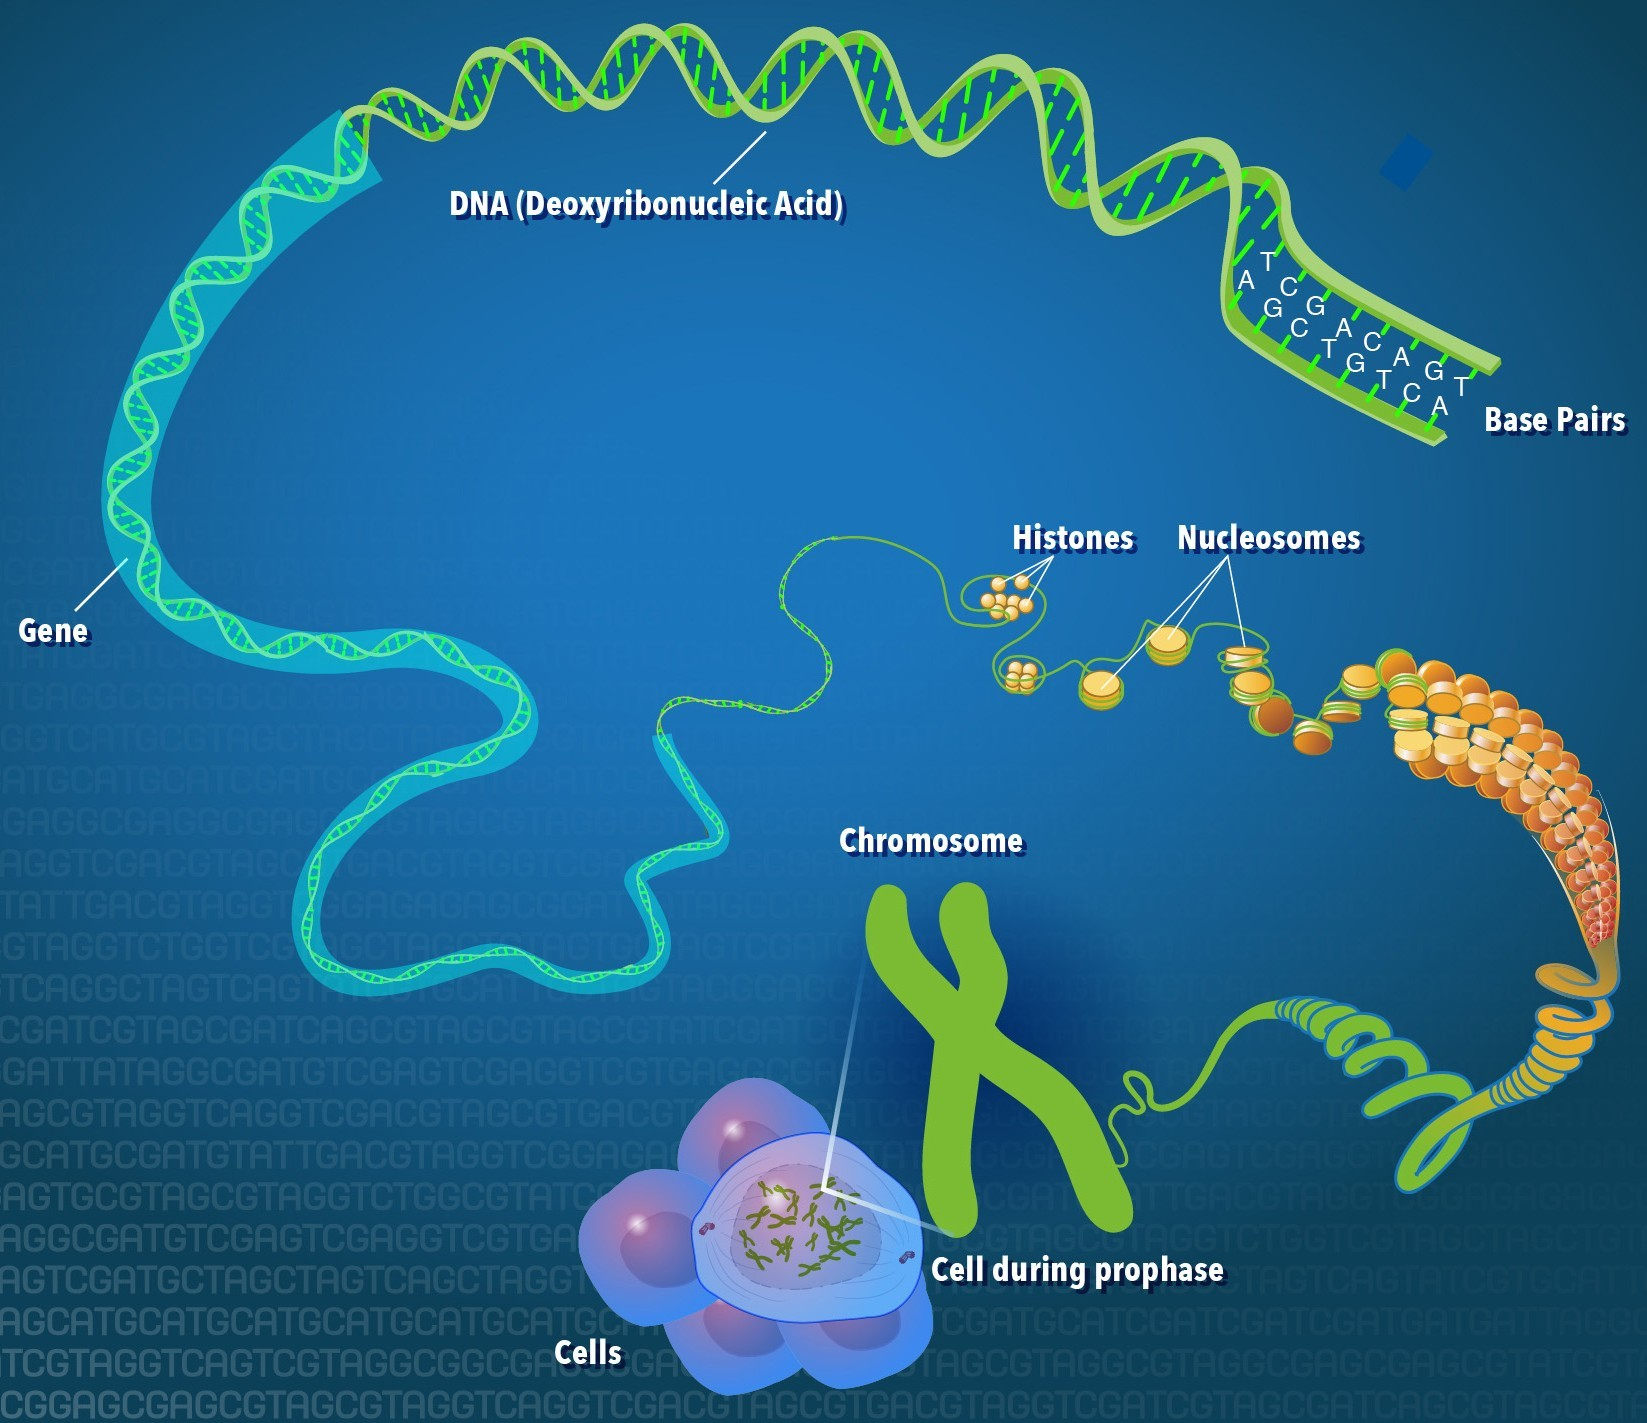
\includegraphics[width=7cm]{c2_gene_01.jpg}}
\begin{enumerate}
  \item 引言与导入(15分钟)\\
    \textcolor{red}{应用还原论引出基因组学涉及的基本概念。}
    \begin{enumerate}
      \item \textcolor{red}{【重点】}基本概念\\
        \textcolor{red}{结合分子生物学知识进行讲解。}
        \begin{itemize}
          \item 基因:DNA上的功能片段
          \item 基因组:一套完整的基因及其调控序列
          \item 基因组学:研究基因组的学科
        \end{itemize}
      \item 基因组
        \begin{itemize}
          \item 构成:常染色体+性染色体+线粒体+叶绿体
          \item 测序:1976,1977,1995,1996,1998
          \item 补遗:基因组构成,基因组大小,基因组演化
        \end{itemize}
    \end{enumerate}

\parpic[fr]{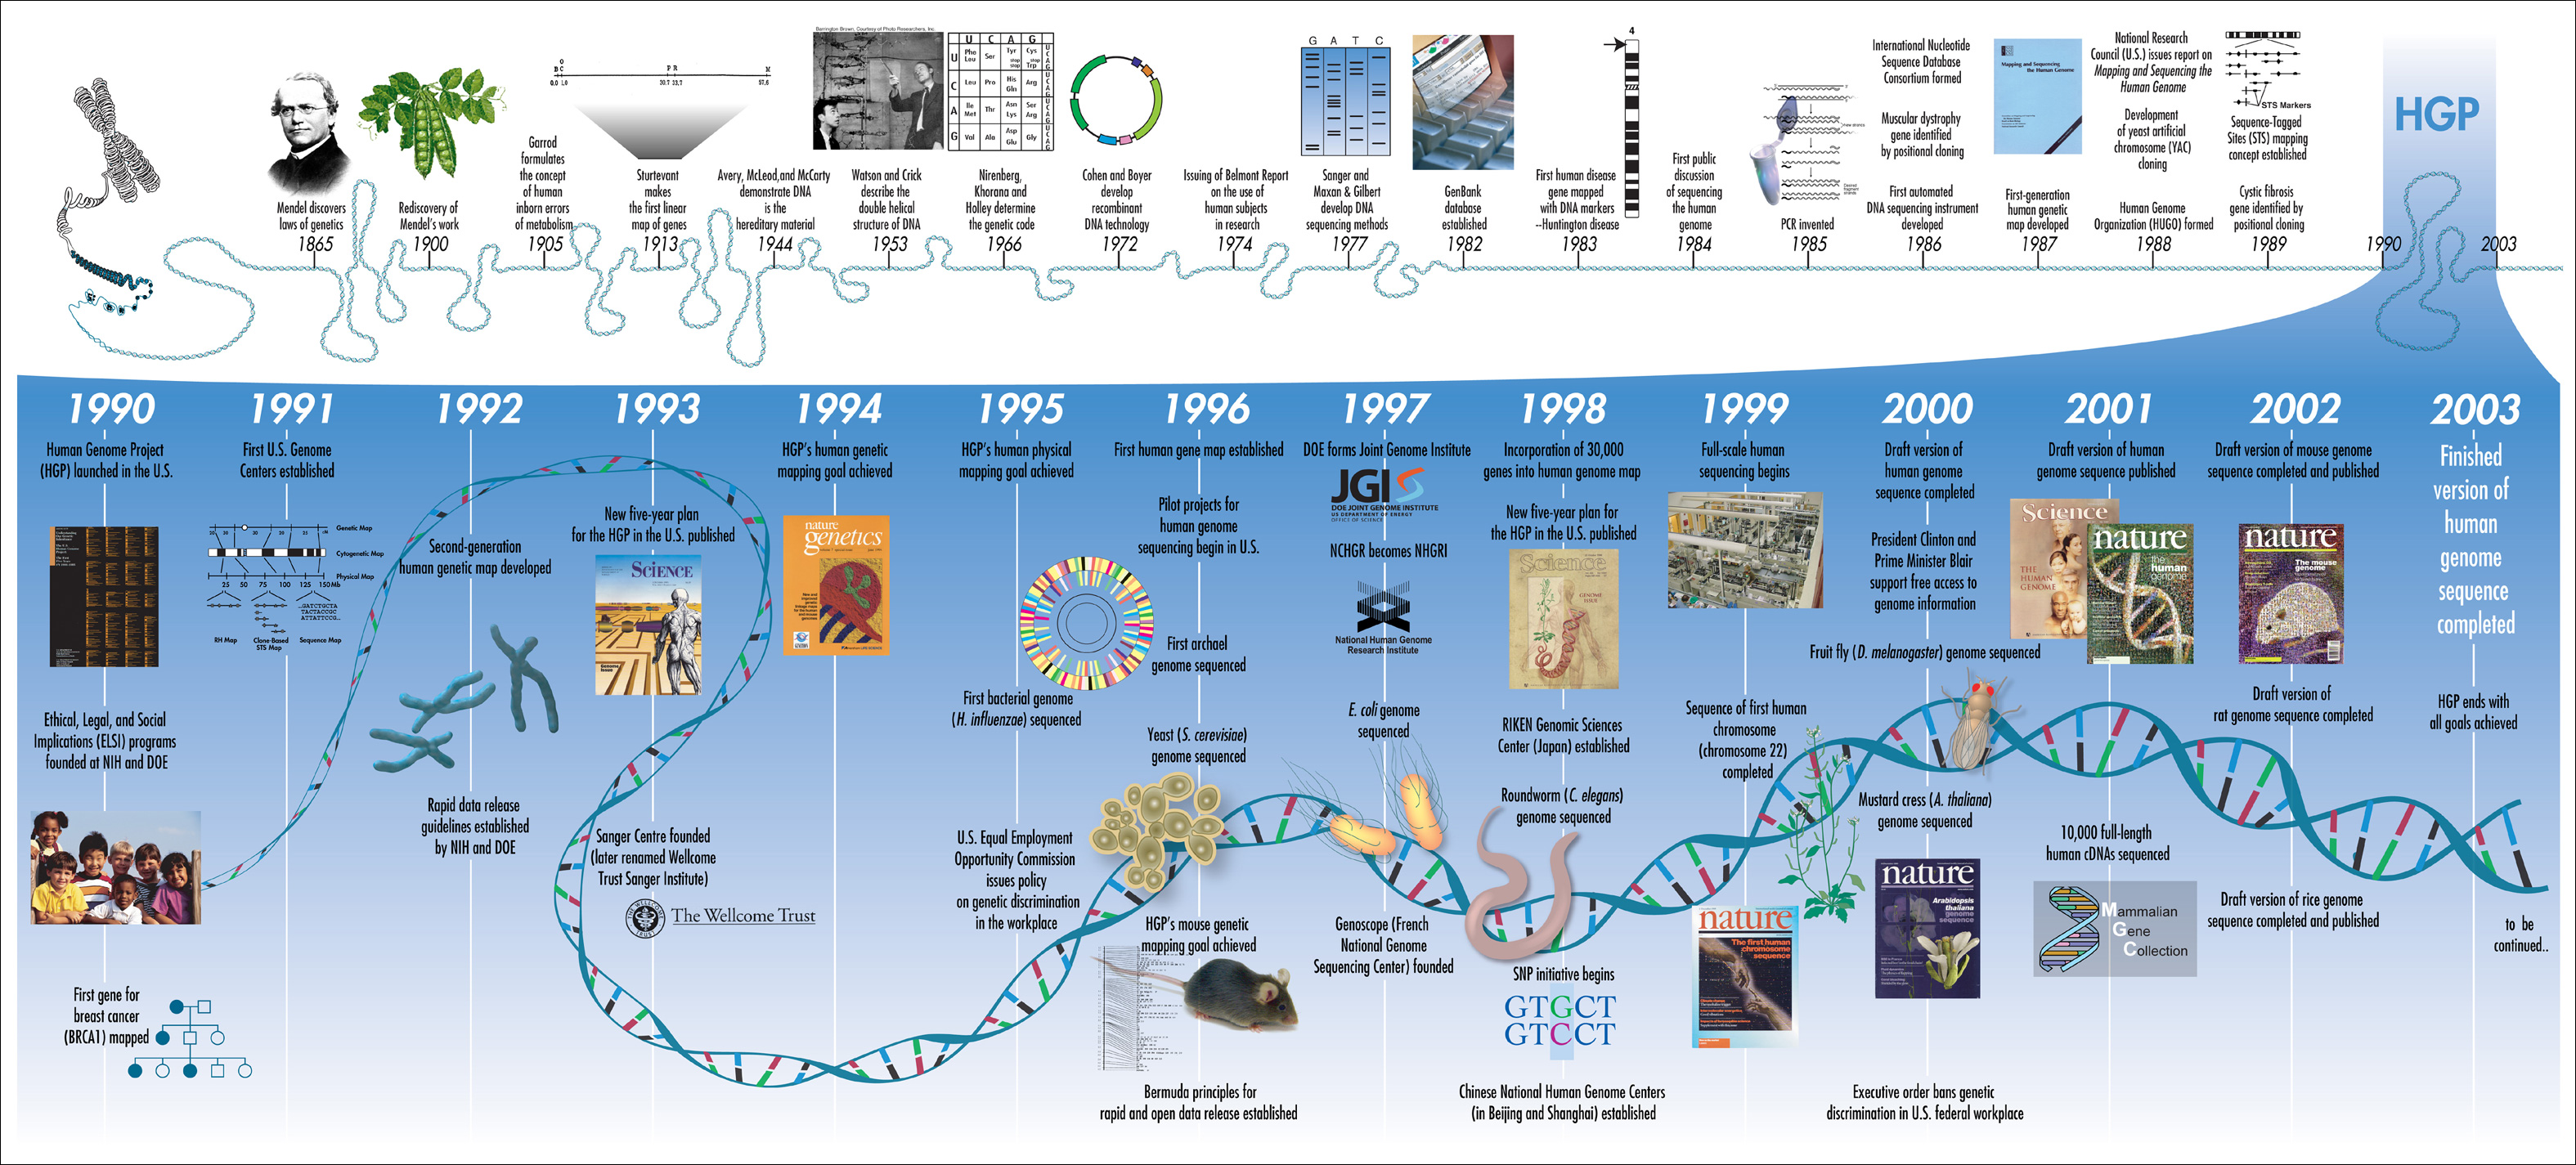
\includegraphics[angle=270,origin=c,width=7cm]{c2_hgp_timeline_01.jpg}}
  \item 人类基因组计划(45分钟)
    \begin{enumerate}
      \item 人类基因组:22+1+1,30亿,~25000
      \item 人类基因组计划(1990~2001)
        \begin{itemize}
          \item 历史事件
          \item \textcolor{red}{【难点】}主要目标\\
            \textcolor{red}{结合人类基因组计划的成果进行讲解。}
            \begin{itemize}
              \item 遗传图谱的绘制
              \item 物理图谱的绘制
              \item 序列测定
              \item 辨别序列中的个体差异
              \item 基因鉴定
              \item 基因的功能性分析
            \end{itemize}
          \item 延伸计划
            \begin{itemize}
              \item 模式生物的基因组计划
              \item 人类元基因组计划
              \item HapMap计划
              \item 人类基因组多样性研究计划
              \item 千人基因组计划
            \end{itemize}
        \end{itemize}
    \end{enumerate}

  \item 基因组学分支学科(35分钟)
    \begin{enumerate}
      \item 结构基因组学:基因组成与定位
      \item 功能基因组学:基因功能和相互作用
      \item 比较基因组学:比较特征和结构
      \item 药物基因组学:精准化医疗
      \item 元基因组:环境微生物群落
    \end{enumerate}

% \otherTail
% \newpage
% \otherHeader

  \item 总结与答疑(5分钟)
    \begin{enumerate}
      \item 知识点
	\begin{itemize}
	  \item 概念:基因、基因组、基因组学
	  \item 人类基因组计划:历史事件、主要目标、延伸计划
	  \item 基因组学分支学科:结构/功能/比较/药物/元基因组
	\end{itemize}
  %     \item 技能
	% \begin{itemize}
	%   \item 
	% \end{itemize}
    \end{enumerate}
\end{enumerate}

\otherTail


\end{document}

